\documentclass{article}
\usepackage[T1]{fontenc}
\usepackage[utf8]{inputenc}
\usepackage{lmodern}
\usepackage[polish,shorthands=off]{babel}
\usepackage{graphicx}
\usepackage{siunitx}
\usepackage{multirow}
\usepackage{longtable}
\usepackage{hyperref}
\usepackage{float}
\usepackage{enumitem}
\title{Sprawozdanie obliczenia naukowe\\Lista 4}
\author{Jakub Kowal}
\date{}
\begin{document}
\maketitle

\section*{Zadania 1--3}
\label{sec:tasks1-3}
\subsection*{Opis zadania}
W zadaniach od 1 do 3 trzeba zaimplementować funkcje:\\
\begin{enumerate}
    \item Obliczającą ilorazy różnicowe.
    \item Obliczającą wartość wielomianu interpolacyjnego stopnia n w postaci Newtona w punkcie $x=t$ za pomocą algorytmu Hornera.
    \item Wyznaczającą współczynniki postaci naturalnej wielomianu interpolacyjnego.
\end{enumerate}
\subsection*{Implementacje}
\begin{enumerate}
    \item W tym zadaniu wykorzystałem rekurencyjne obliczanie ilorazów różnicowych w taki sam sposób jak występowało to na \href{https://cs.pwr.edu.pl/zielinski/lectures/scna/scnaw6.pdf#page=16}{slajdach z wykładu}. 
    \item Zadanie 2 wykorzystuje wzór na algorytm Hornera podany w \href{https://cs.pwr.edu.pl/zielinski/lectures/scna/scnal4cw.pdf#page=2}{zadaniu 8 na liście 4}.
    \item To zadanie sprawiło najwięcej kłopotów. Oznaczając ilorazy różnicowe $c_{n}=f_{[x_{0},x_{1},\dots,x_{n}]}$ korzystamy z tego, że $c_{n}\text{=}a_{n}$, gdzie $a_{n}$ jest współczynnikiem przy największej potędze w naturalnej postaci wielomianu. Następnie liczymy w tablicy $a$ wartości "aktualnego wielomianu" (Korzystamy z algorytmu Hornera w celu rozwinięcia aktualnego wielomianu) i na początku tablicy ustawiamy aktualny wyraz wolny.
\end{enumerate}

\section*{Zadanie 4}
\label{sec:task4}
\subsection*{Opis zadania}
Zadanie polega na napisaniu funkcji interpolującej podaną funkcję $f(x)$, za pomocą wielomianu interpolacyjnego stopnia $n$ w postaci Newtona w przedziale $[a,b]$. W tym celu mamy użyć wcześniej zaimplementowanych funkcji. W dodatku funkcja ta ma rysować wielomian interpolacyjny oraz interpolowaną funkcję w podanym przedziale. Funkcja w tym zadaniu ma na celu stworzenie i zwrócenie wykresu (w celu podstawienia opisów do wykresów przy wywołaniu testu) i wyznaczenie węzłów wielomianu interpolacyjnego dwoma różnymi metodami.
\subsection*{Implementacja}
Najpierw wyznaczamy węzły interpolacji metodą doprecyzowaną w wywołaniu funkcji. Mamy dwie możliwe do wywołania metody: 
\begin{itemize}
    \item :rownoodlegle
    \item :czebyszew
\end{itemize}
Równoodległe wyznaczane są prostym wzorem: $x_{k} = a + k\frac{b-a}{n} \text{ dla } k\in [0,n]$.\\
Wyznaczanie węzłów metodą wielomianu Czebyszewa jest trochę bardziej problematyczne. Wzór na miejsca zerowe wielomianu Czebyszewa stopnia $n$ podany na \href{https://cs.pwr.edu.pl/zielinski/lectures/scna/scnaw7.pdf#page=8}{wykładzie}: $r_{j}=\cos\frac{(2j+1)\pi}{2n} \text{ dla } j\in [0,n-1]$ zwraca pierwiastki jedynie z przedziału [-1,1], więc trzeba te pierwiastki zmapować na podany przedział [a,b].\

\section*{Zadanie 5}
\label{sec:task5}
\subsection*{Opis zadania}
Należy użyć wcześniej zadeklarowanej funkcji \textit{rysujNnfx} z \hyperref[sec:task4]{zadania 4} dla funkcji:\\
\begin{enumerate}[label=\alph*)]
    \item $f(x)=e^{x}$
    \item $x^{2}\sin x$
\end{enumerate}
Dla stopni wielomianu $n \in {5,10,15}$
\subsection*{Wyniki}
Wyniki dla funkcji $e^{x}$
\begin{figure}[H]
    \label{fig:Z5_a_5}
    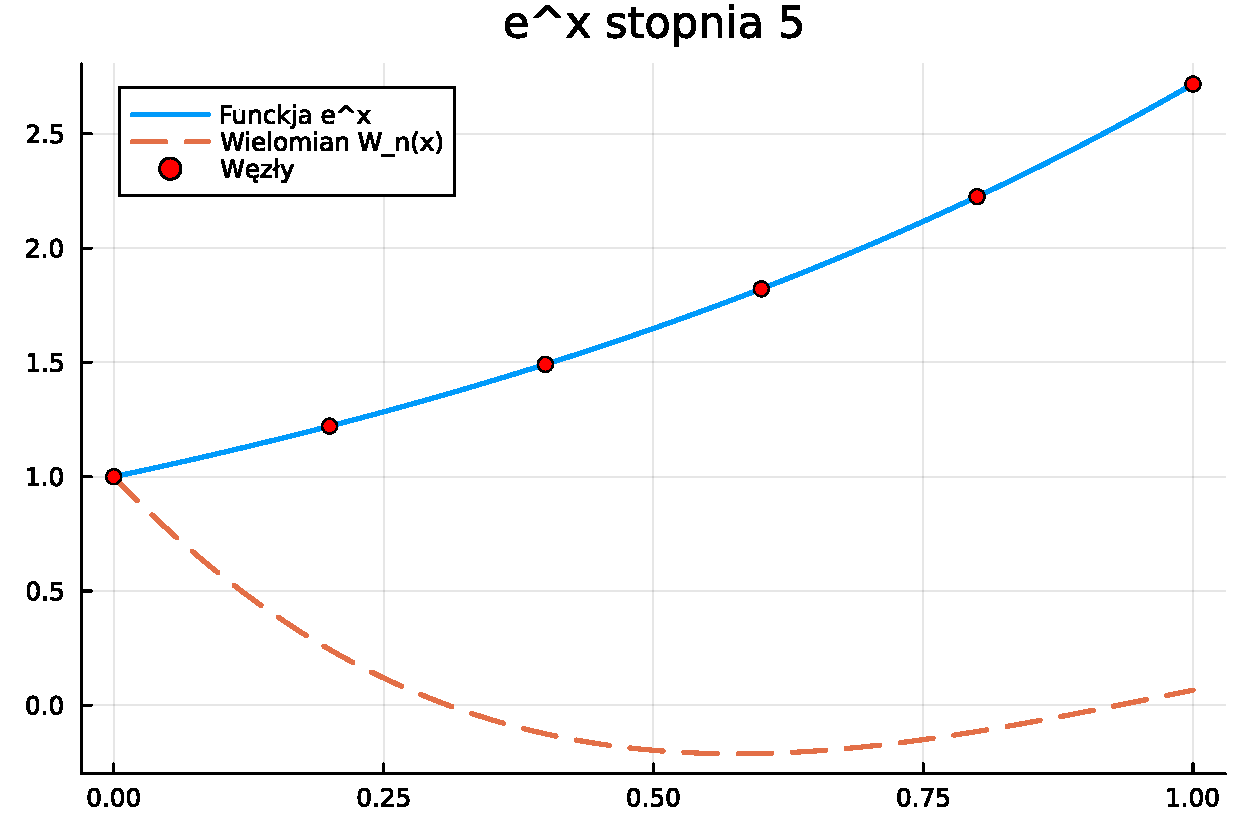
\includegraphics[width=35em]{Plots/Z5_a_5.pdf}
\end{figure}
\begin{figure}[H]
    \label{fig:Z5_a_10}
    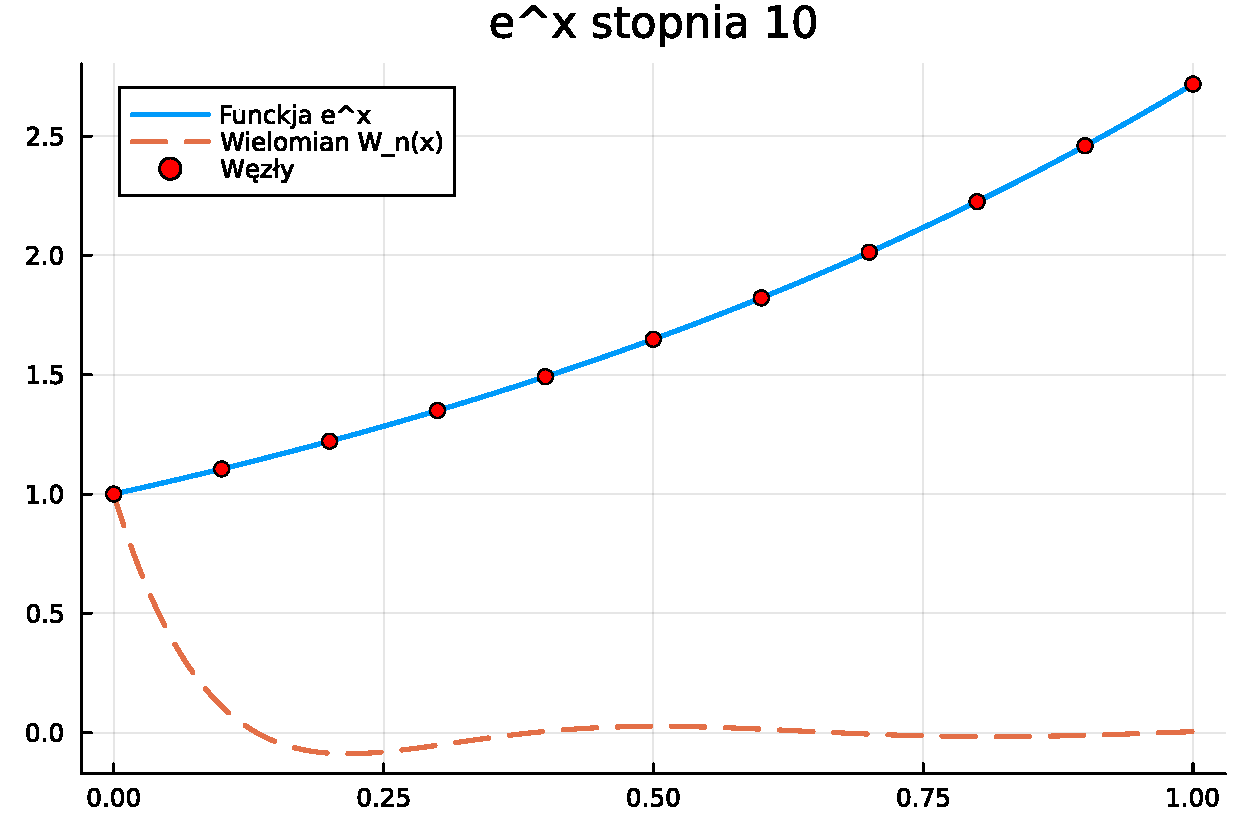
\includegraphics[width=35em]{Plots/Z5_a_10.pdf}
\end{figure}
\begin{figure}[H]
    \label{fig:Z5_a_15}
    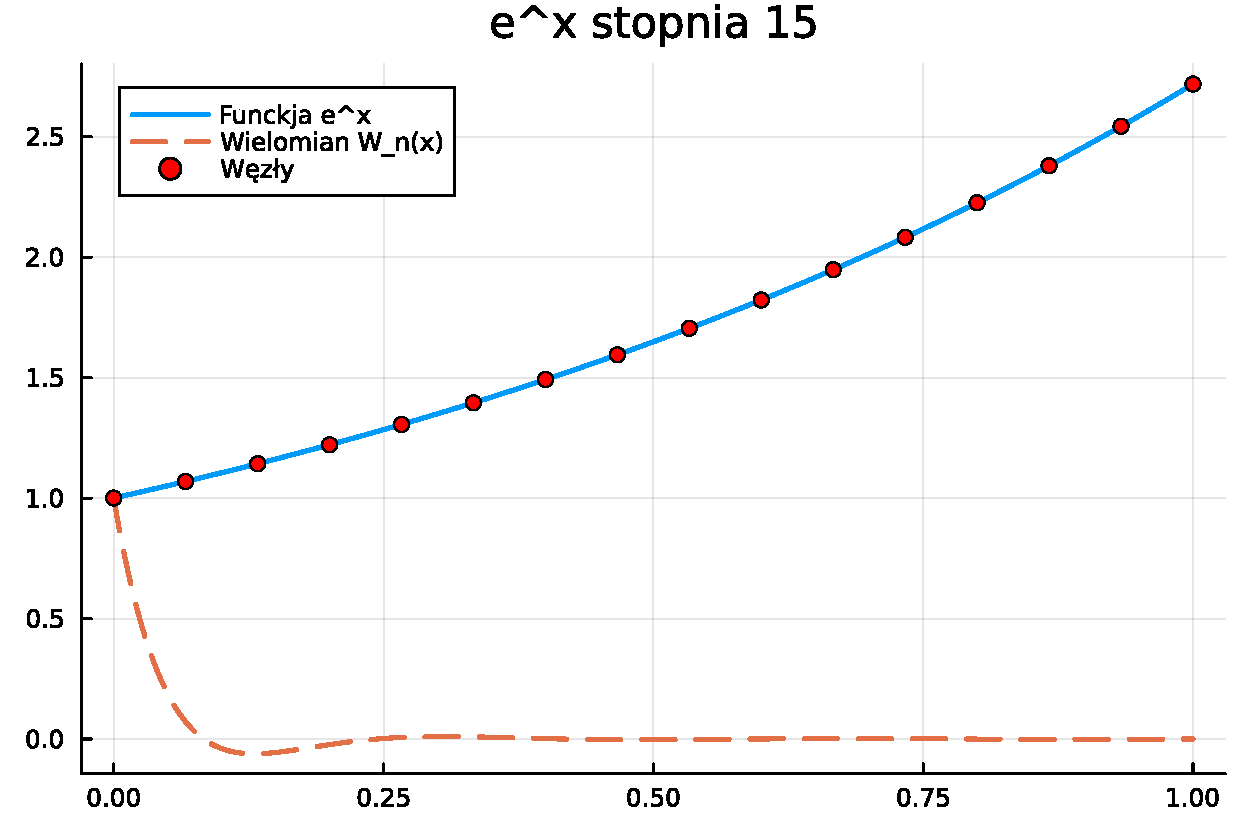
\includegraphics[width=35em]{Plots/Z5_a_15.pdf}
\end{figure}
Wyniki dla funkcji $x^{x}\sin x$
\begin{figure}[H]
    \label{fig:Z5_b_5}
    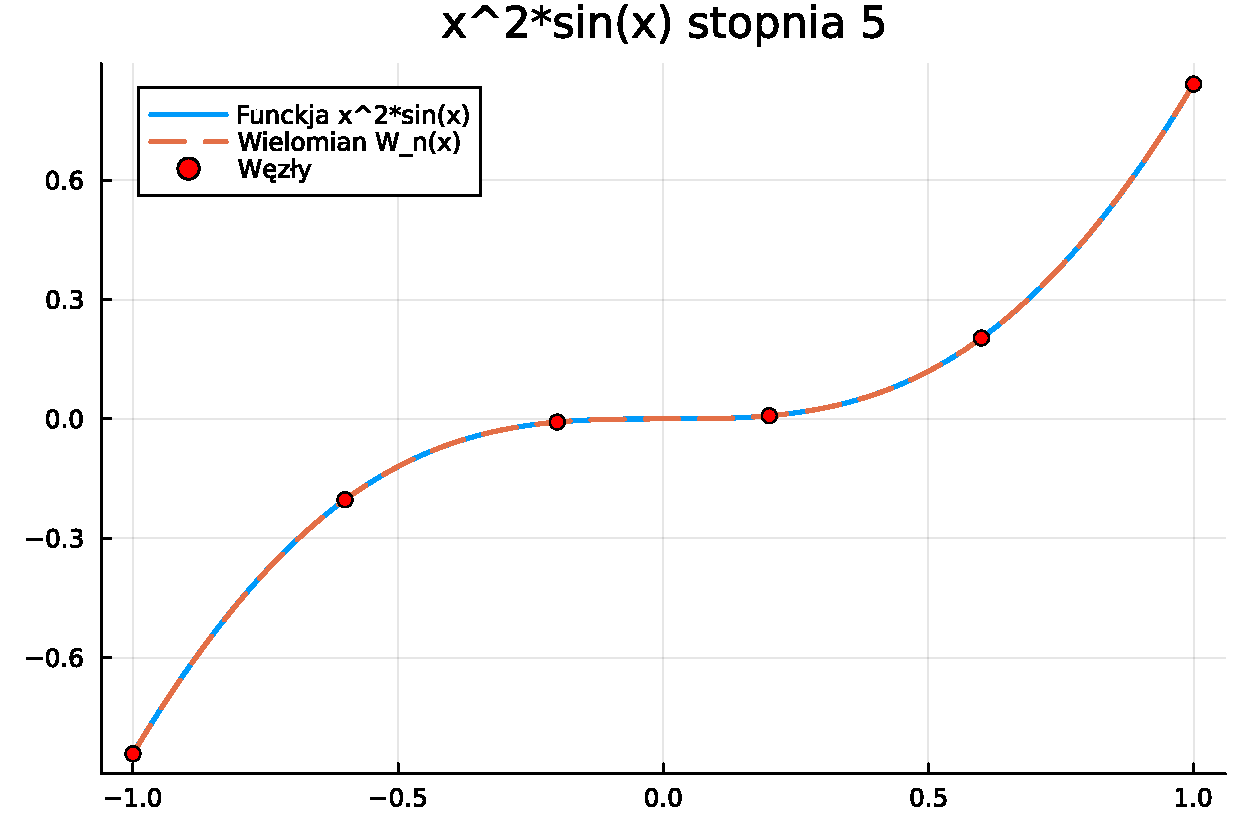
\includegraphics[width=35em]{Plots/Z5_b_5.pdf}
\end{figure}
\begin{figure}[H]
    \label{fig:Z5_b_10}
    \includegraphics[width=35em]{Plots/Z5_b_10.pdf}
\end{figure}
\begin{figure}[H]
    \label{fig:Z5_b_15}
    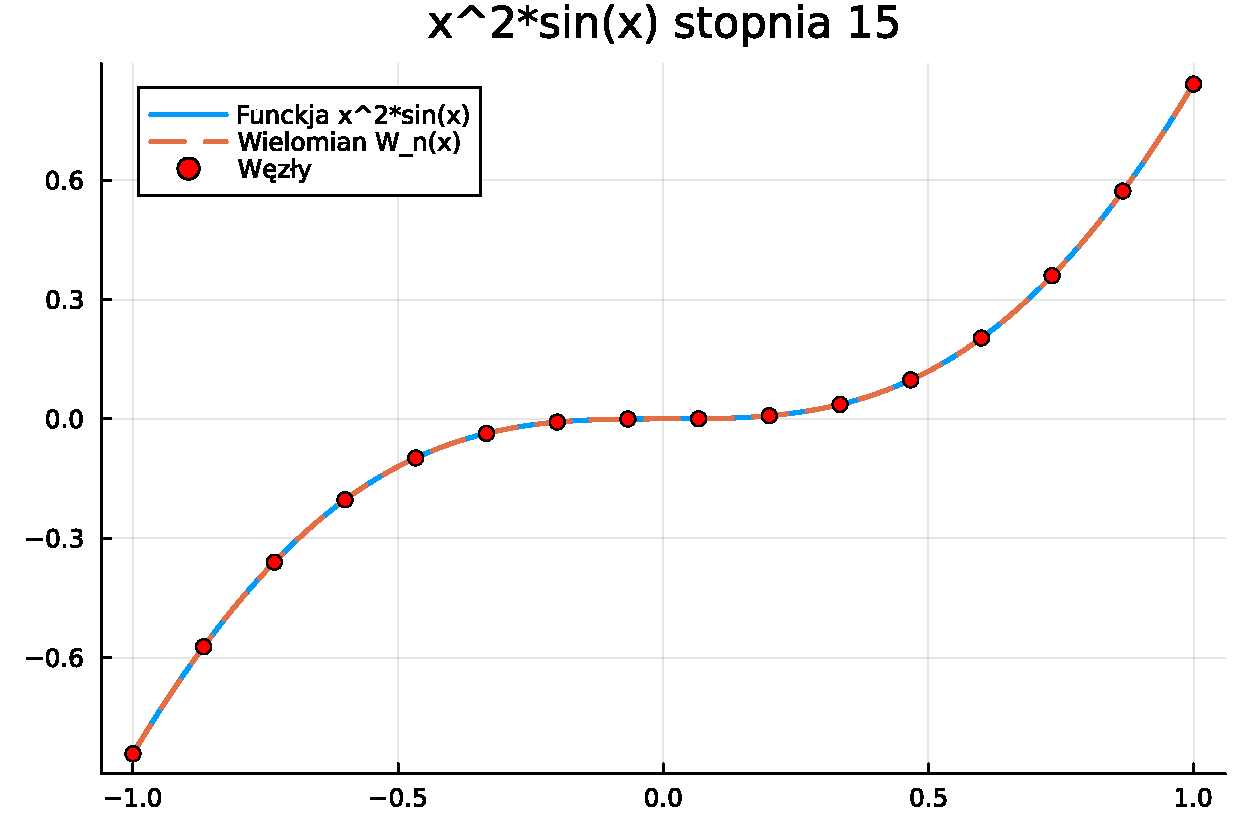
\includegraphics[width=35em]{Plots/Z5_b_15.pdf}
\end{figure}

\subsection*{Wnioski}
Jak widać na powyższych wykresach wartość interpolacji pokrywa się wręcz z wykresami funkcji, więc spokojnie można określić interpolację, jako bardzo precyzyjne przybliżenie funkcji.

\section*{Zadanie 6}
\label{sec:task6}
\subsection*{Opis zadania}
W tym zadaniu trzeba przetestować funkcje $f(x)=|x| \text{ oraz } \frac{1}{1+x^{2}}$ dla różnych stopni wielomianu interpolującego, jak i dla dwóch sposobów wyznaczania węzłów. Dla przykładu a przedziałem będzie [-1,1], a dla b [-5,5].

\subsection*{Wyniki}

Wyniki dla $f(x)=|x|$ w przedziale [-1,1], wyznaczając węzły równoodległe:

\begin{figure}[H]
    \label{fig:Z6_a_r_5}
    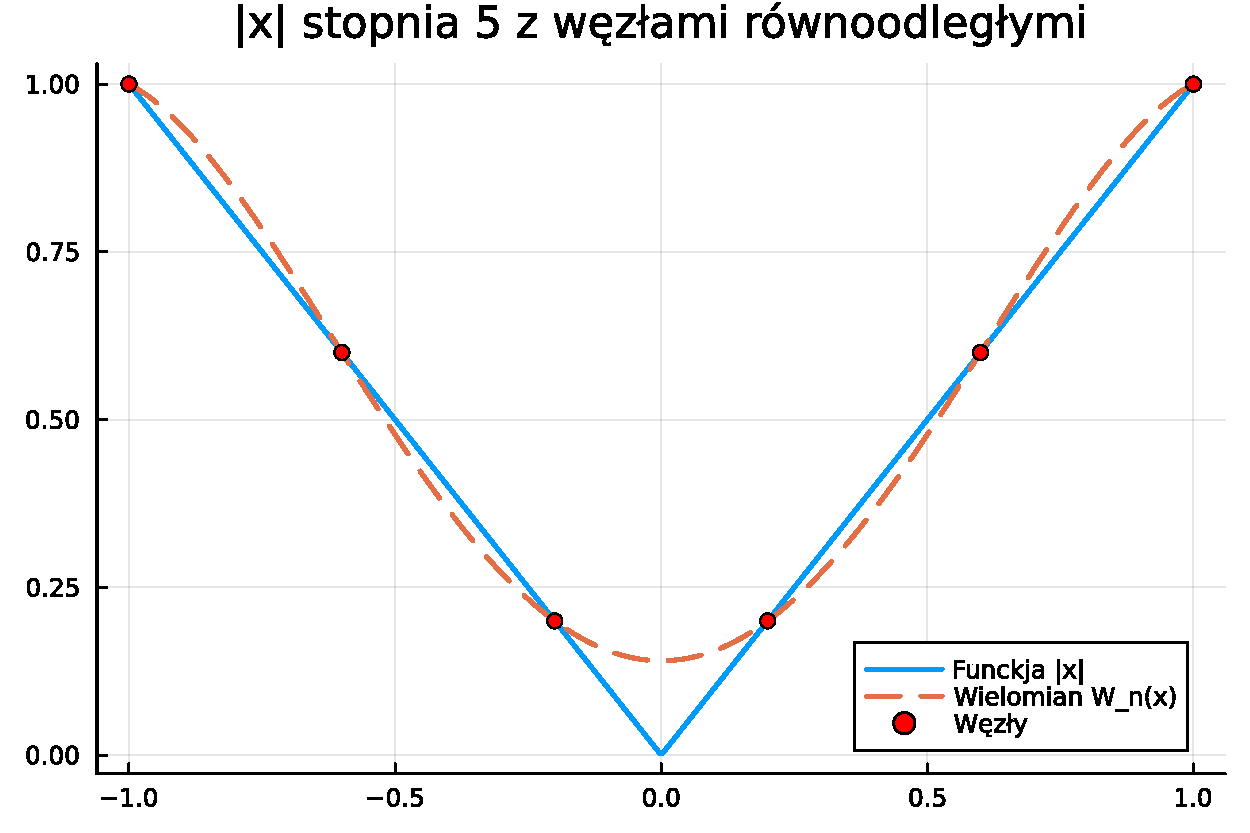
\includegraphics[width=35em]{Plots/Z6_a_r_5.pdf}
\end{figure}
\begin{figure}[H]
    \label{fig:Z6_a_r_10}
    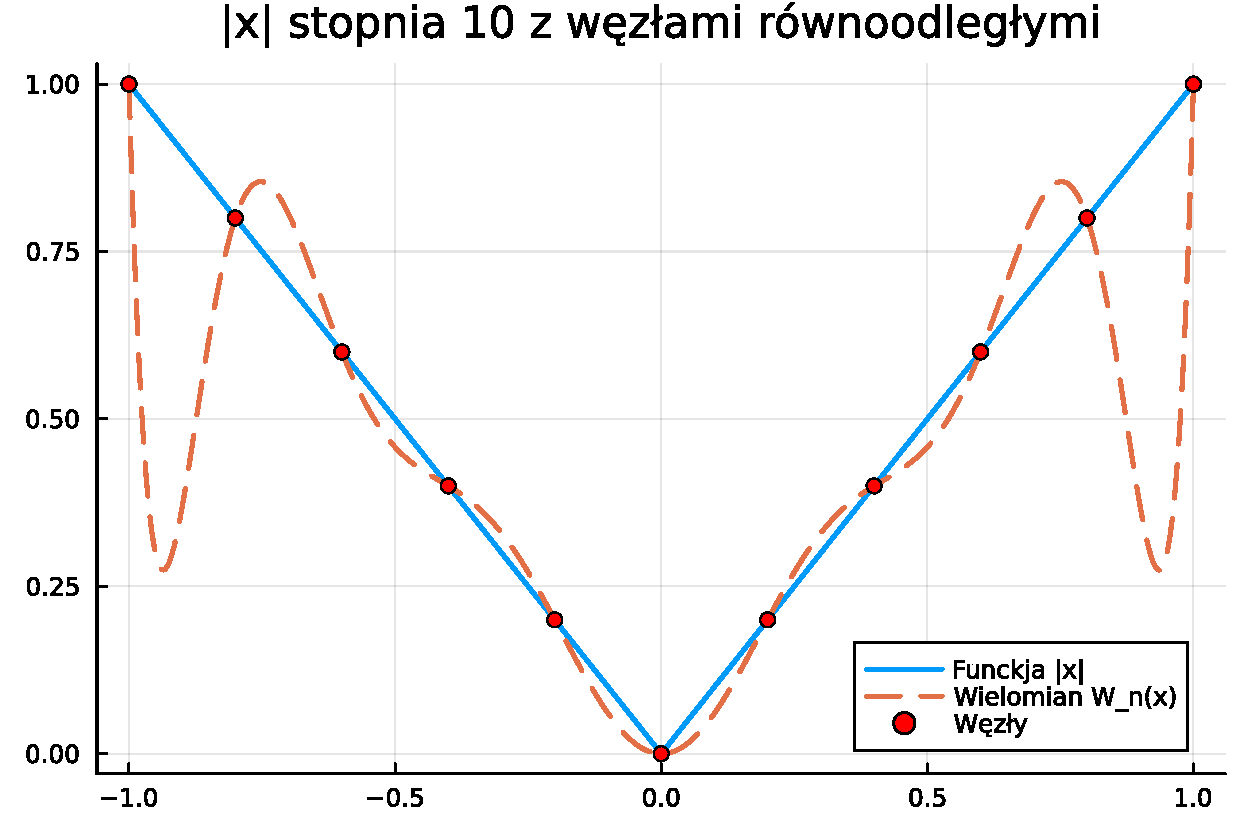
\includegraphics[width=35em]{Plots/Z6_a_r_10.pdf}
\end{figure}
\begin{figure}[H]
    \label{fig:Z6_a_r_15}
    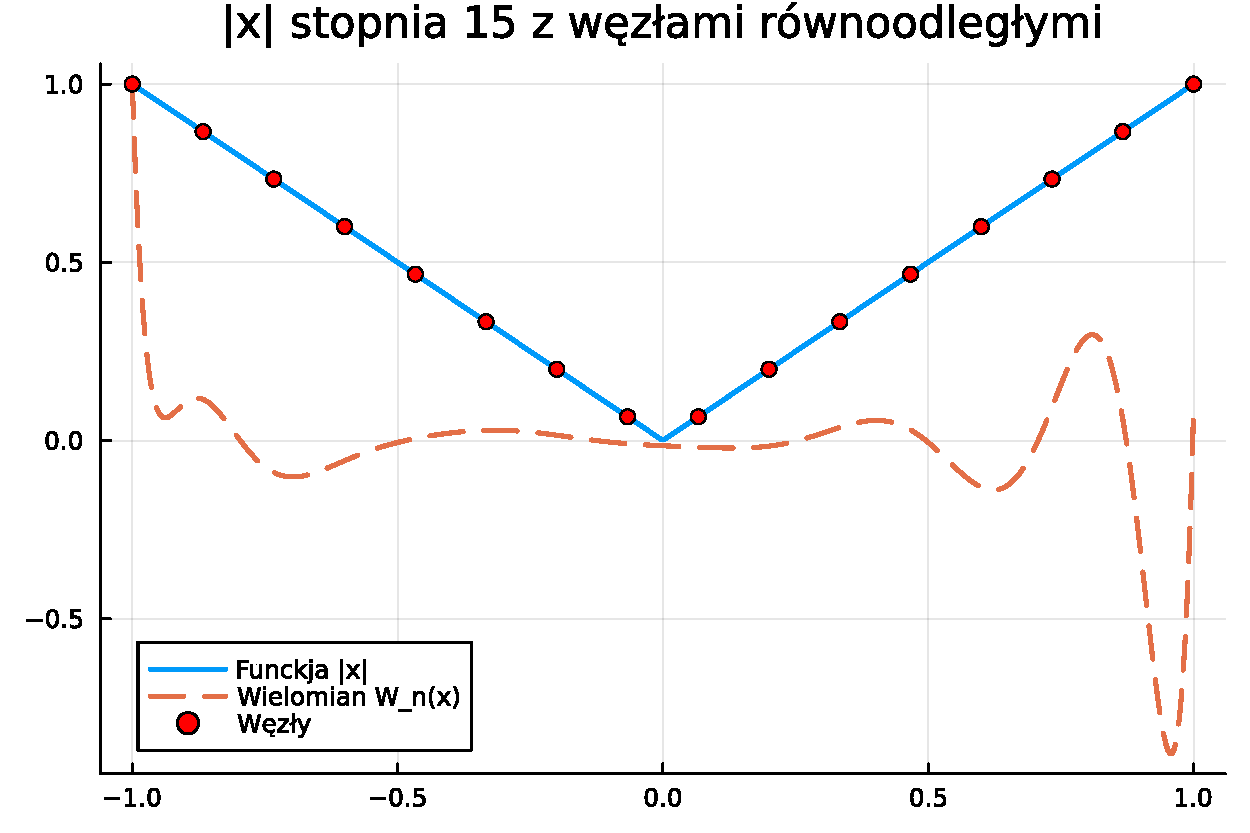
\includegraphics[width=35em]{Plots/Z6_a_r_15.pdf}
\end{figure}

Wyniki dla $f(x)=|x|$ w przedziale [-1,1] biorąc za węzły zera wielomianu Czebyszewa:

\begin{figure}[H]
    \label{fig:Z6_a_c_5}
    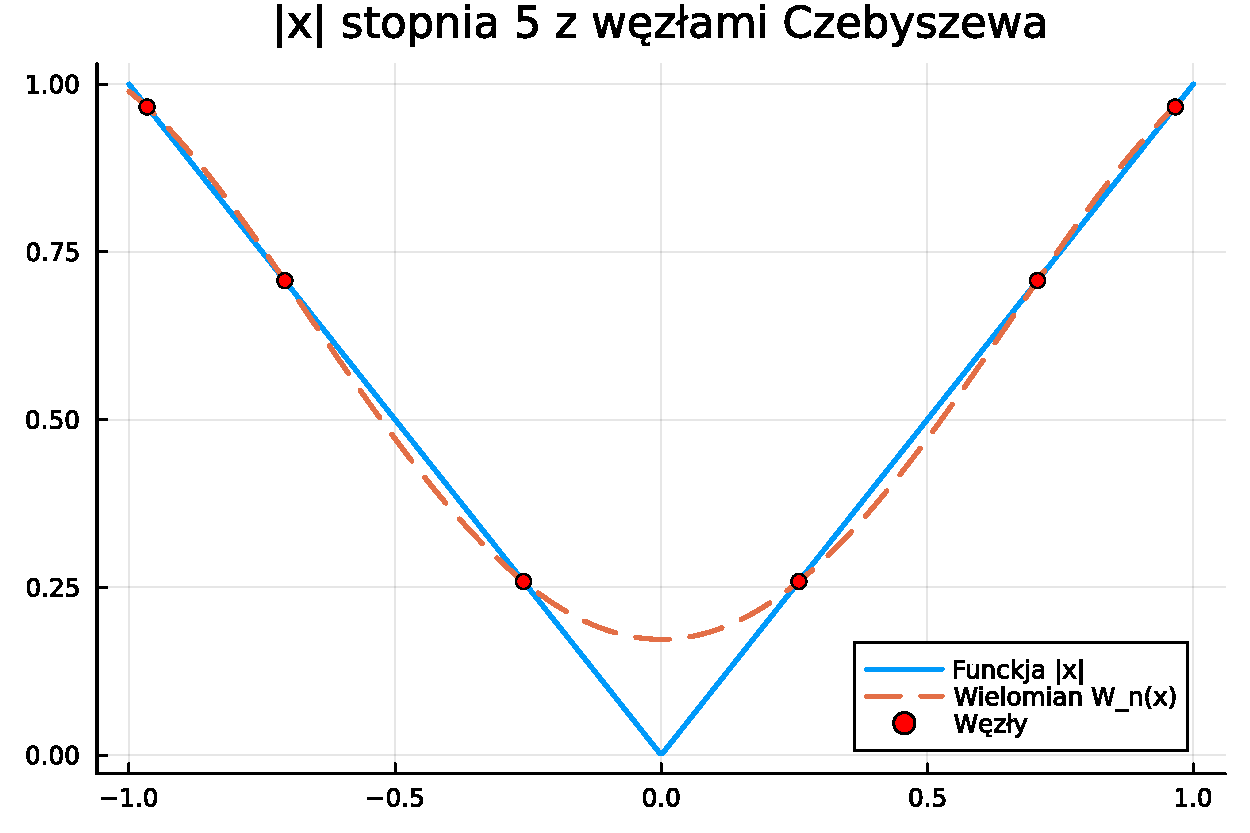
\includegraphics[width=35em]{Plots/Z6_a_c_5.pdf}
\end{figure}
\begin{figure}[H]
    \label{fig:Z6_a_c_10}
    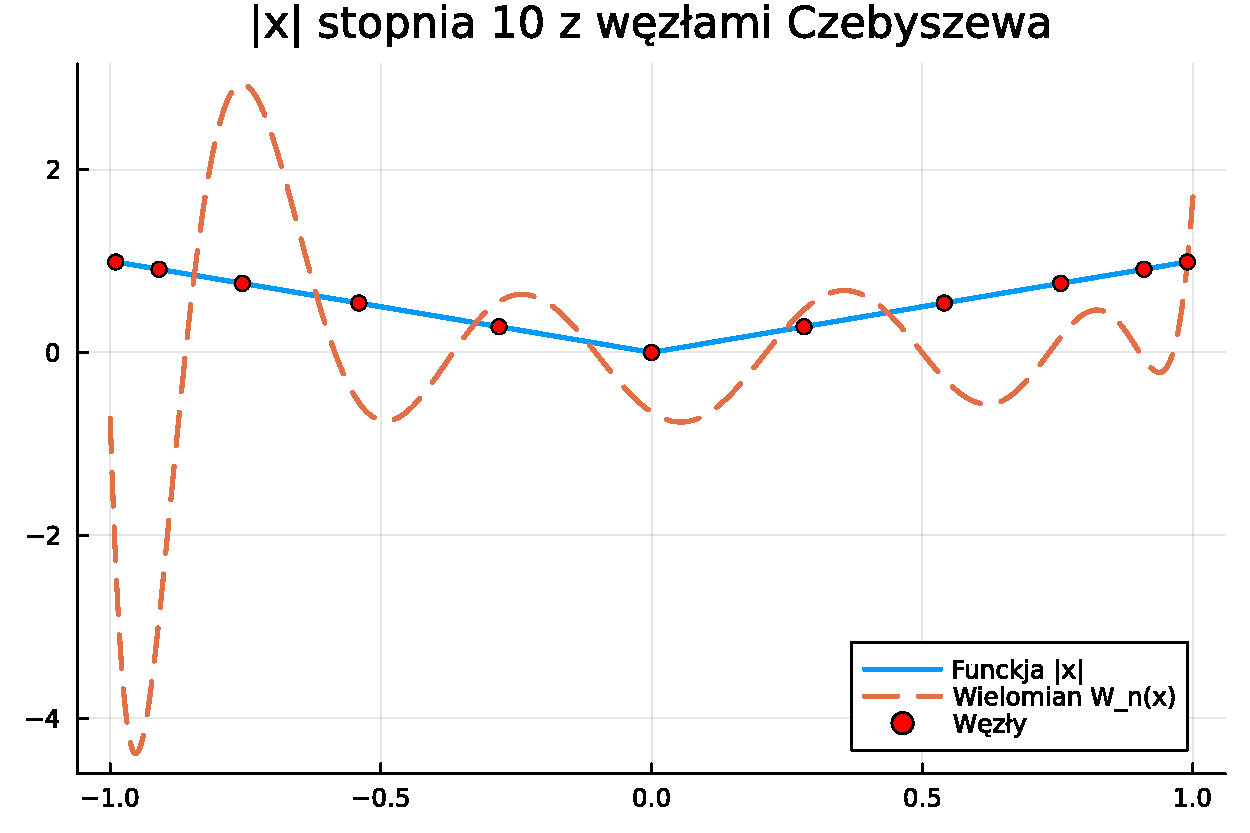
\includegraphics[width=35em]{Plots/Z6_a_c_10.pdf}
\end{figure}
\begin{figure}[H]
    \label{fig:Z6_a_c_15}
    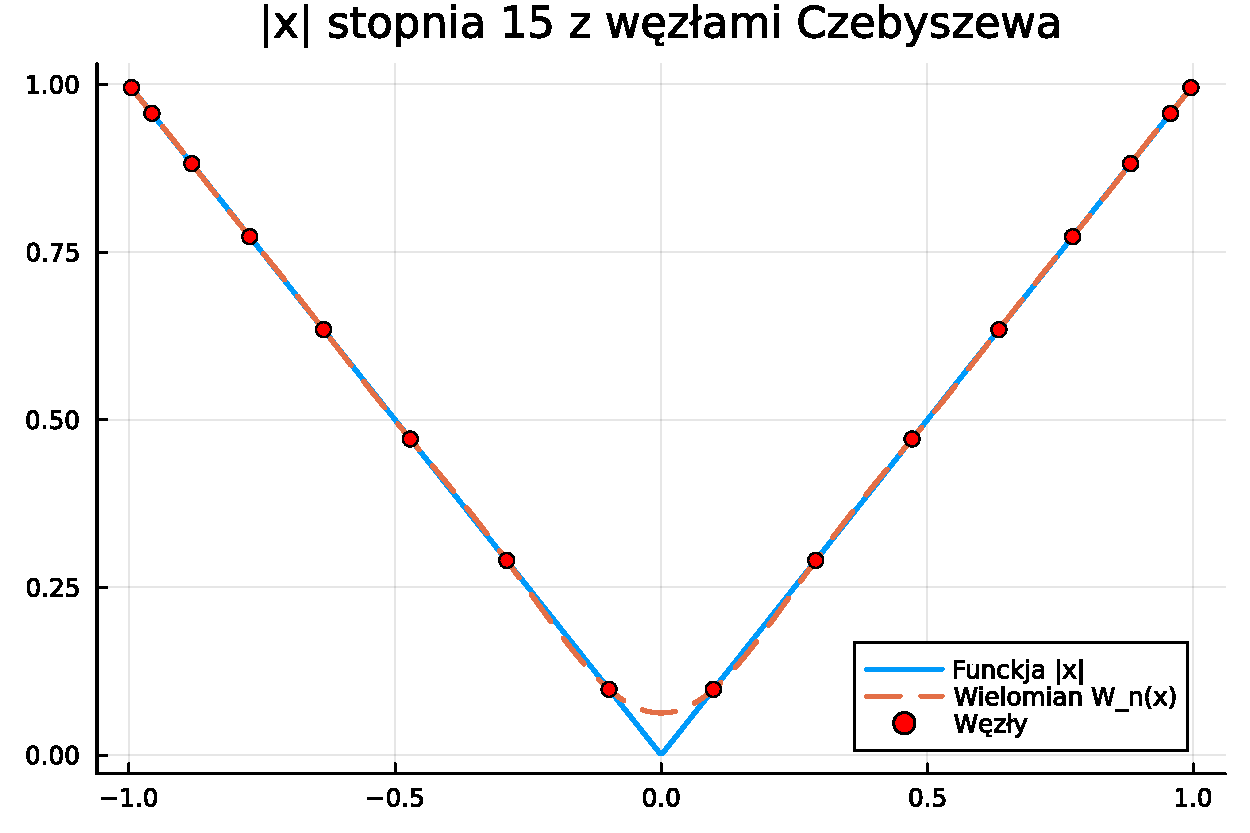
\includegraphics[width=35em]{Plots/Z6_a_c_15.pdf}
\end{figure}

Wyniki dla $f(x)=\frac{1}{1+x^{2}}$ w przedziale [-5,5], wyznaczając węzły równoodległe:

\begin{figure}[H]
    \label{fig:Z6_b_r_5}
    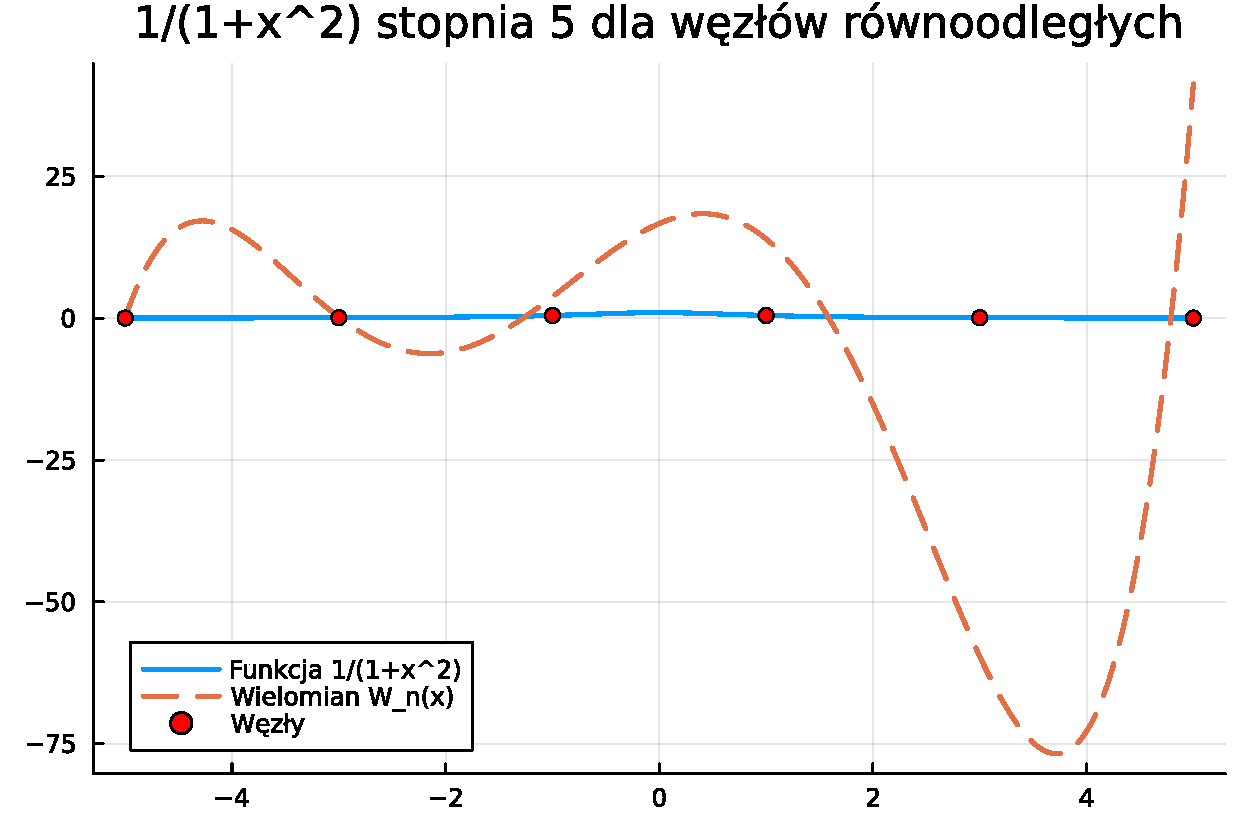
\includegraphics[width=35em]{Plots/Z6_b_r_5.pdf}
\end{figure}
\begin{figure}[H]
    \label{fig:Z6_b_r_10}
    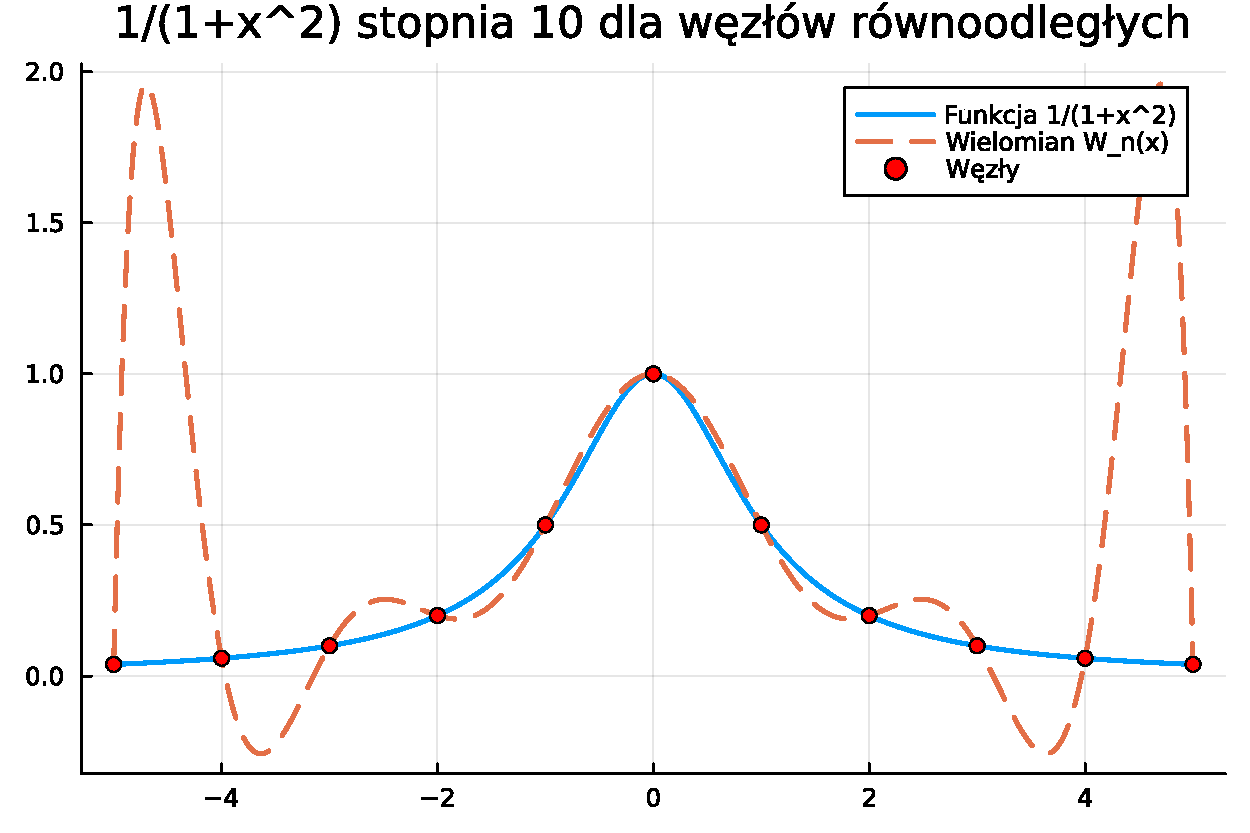
\includegraphics[width=35em]{Plots/Z6_b_r_10.pdf}
\end{figure}
\begin{figure}[H]
    \label{fig:Z6_b_r_15}
    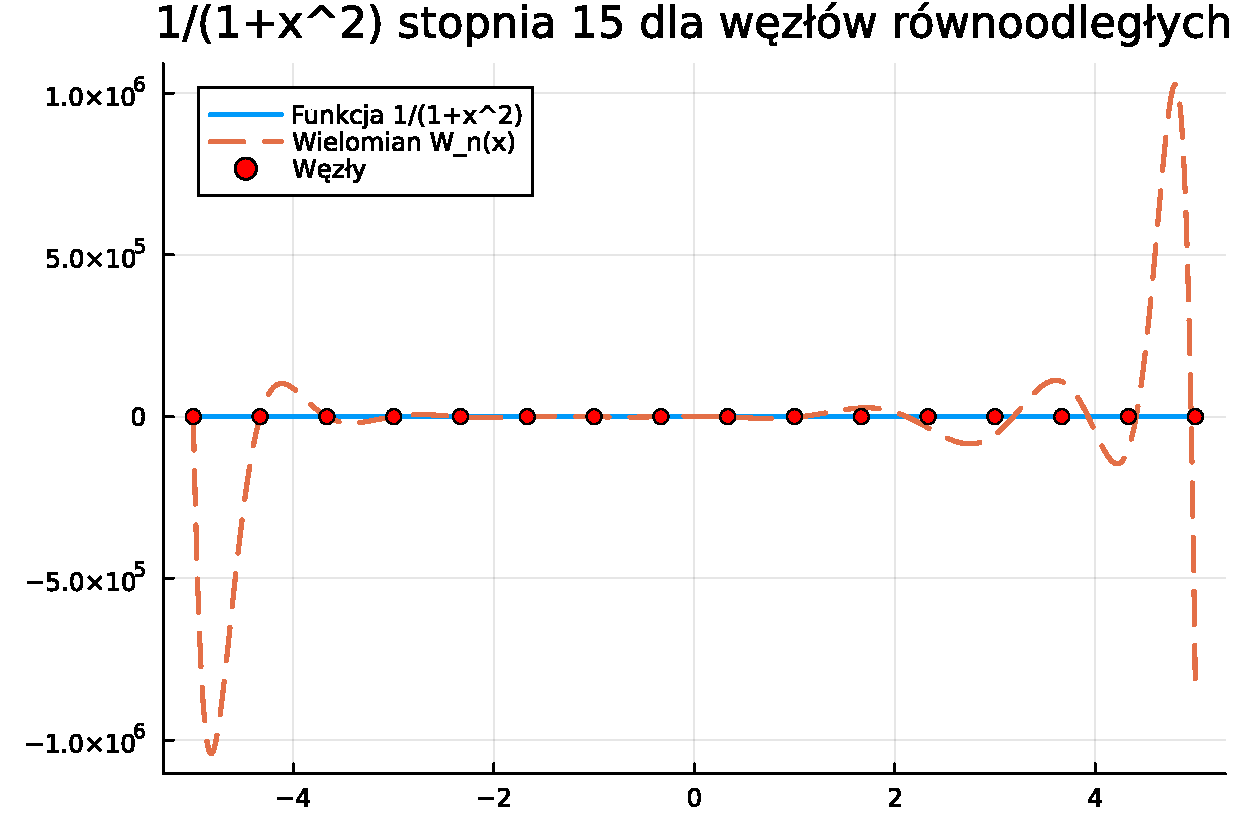
\includegraphics[width=35em]{Plots/Z6_b_r_15.pdf}
\end{figure}

Wyniki dla $f(x)=\frac{1}{1+x^{2}}$ w przedziale [-5,5] biorąc za węzły zera wielomianu Czebyszewa:

\begin{figure}[H]
    \label{fig:Z6_b_c_5}
    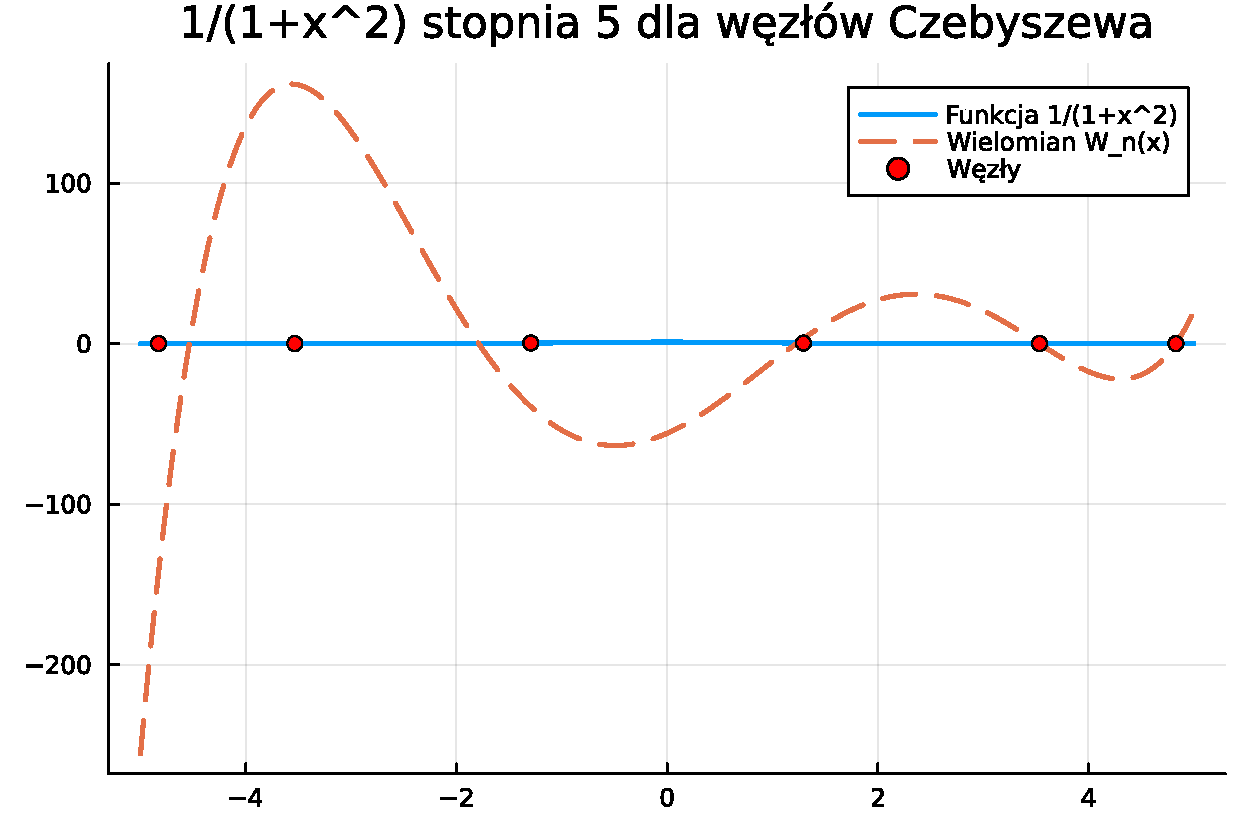
\includegraphics[width=35em]{Plots/Z6_b_c_5.pdf}
\end{figure}
\begin{figure}[H]
    \label{fig:Z6_b_c_10}
    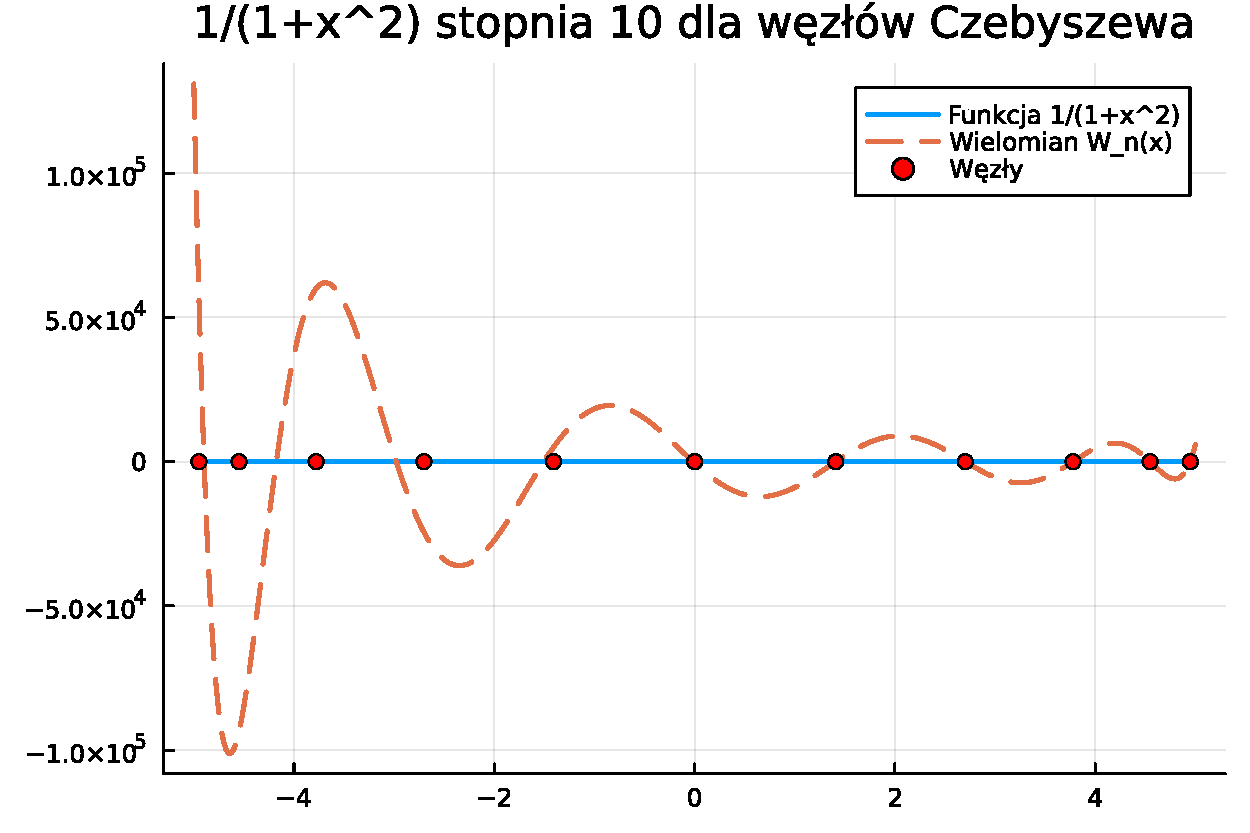
\includegraphics[width=35em]{Plots/Z6_b_c_10.pdf}
\end{figure}
\begin{figure}[H]
    \label{fig:Z6_b_c_15}
    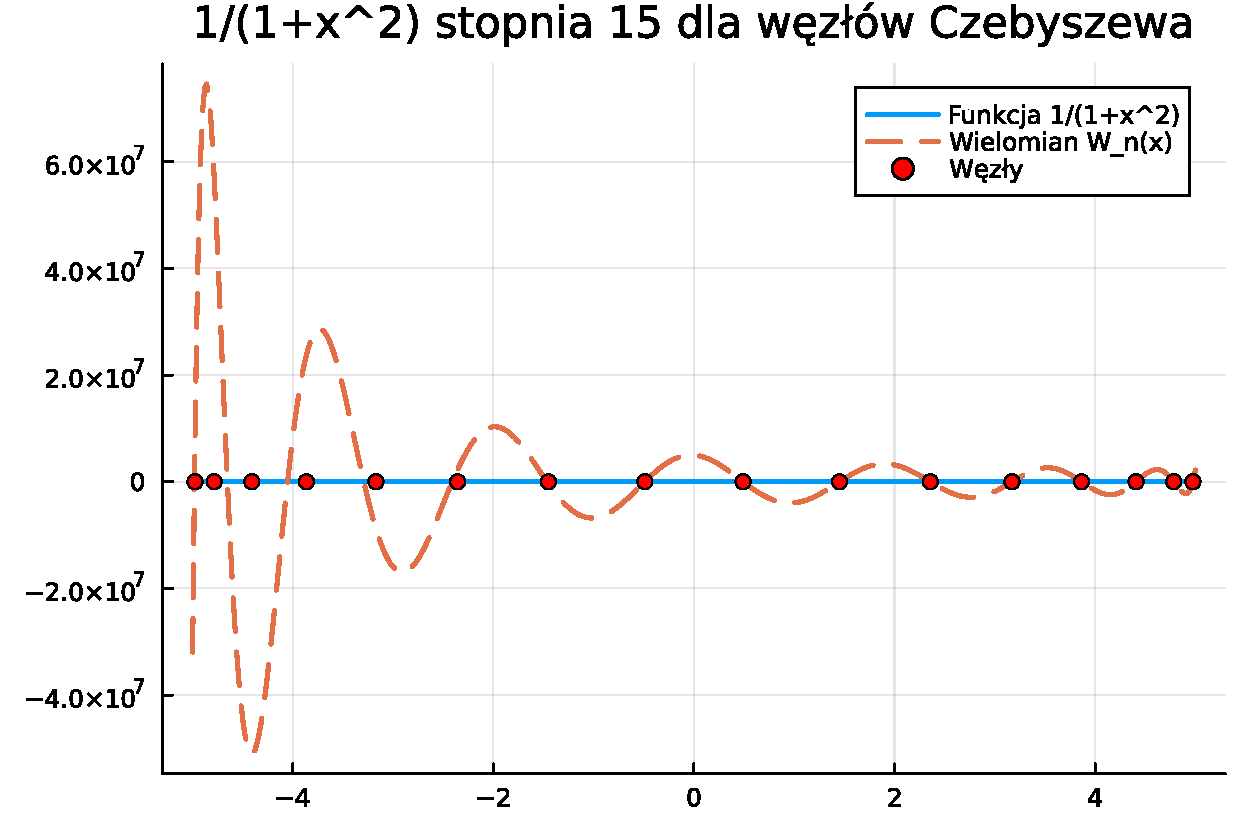
\includegraphics[width=35em]{Plots/Z6_b_c_15.pdf}
\end{figure}

\subsection*{Wnioski}
Jak widać na załączonych wykresach wybieranie węzłów co równą odległość ma swoje wady. Na wykresach z węzłami równoodległymi w tym zadaniu ukazuje nam się zjawisko Runge'go. Powoduje ono coraz większe błędy przy coraz większych stopniach wielomianu interpolacyjnego, zwłaszcza na brzegach rozważanego przedziału. \colorbox{yellow}{Placeholder ( dopisać coś do zjawiska Runge'go)}. Można zapobiedz takim wahaniom wybierając węzły za pomocą miejsc zerowych wielomianu Czebyszewa. Powoduje to badziej "gęste" dobieranie punktów na brzegach przedziału i niweluje wahania widoczne w zjawisku Runge'go.


\end{document}